\documentclass[12pt]{article}

\usepackage{uw_rpt} 				% Template from Github.com/patrickkang/uwaterloo_wkrpt
\usepackage{graphicx} 				% Formatting of figures
\usepackage{amsmath}				% Only used for Greek symbols
\usepackage{array}					% More options for tables
\usepackage{verbatim}				% I forget why this is required, but it is
\usepackage{minted} 				% For code examples in appendix A
\usepackage{finstrut}				% Scared to delete this one too
\usepackage{apacite} 				% Better APA format than the default
\usepackage{url} 					% Makes Github URLs look nice
\usepackage[section]{placeins} 		% Fixes placement of floats
\usepackage[labelfont=bf]{caption} 	% Makes "Figure x:" bold

% Fixes issue of the table being labelled as a figure
\def\table{\def\figurename{Table}\figure}
\let\endtable\endfigure 

\begin {document}

% \UWtitle{report title} { workplace } {Name and Date} %
\UWtitle{Uncovering Patterns of Cyanobacteria Diversification using Kaphi}
{
	Schulich School of Medicine \& Dentistry\\
	London, ON
	}{
	Mathias Renaud\\
	ID 20558745\\
	3B Biology \\
	\today
}


% ABSTRACT LETTER %
\begin{UWletter}
\thispagestyle{empty}
Mathias Renaud\\
334 Lester St.\\
Waterloo, Ontario\\
N2L 3W7\\
\\
\today\\
\\
Dr. Hugh Broders\\
Department of Biology\\
University of Waterloo\\
Waterloo, Ontario\\
N2L 3G1\\
\\
Dear Dr. Hugh Broders,\\
\\
This report, entitled ``Uncovering Patterns of Cyanobacteria Diversification using Kaphi'' was prepared for Schulich School of Medicine and Dentistry. This is my third work report, which was completed following my 3A term.  The aim of this report is to investigate the diversification rates of the cyanobacteria clade by analyzing a comprehensive phylogeny with the phylodynamic software package, Kaphi.

I was a member of the Poon Lab, headed by Dr. Art Poon, within the department of Pathology and Laboratory Medicine. The lab develops bioinformatics software, with a focus on tools for characterizing the patterns of epidemics.

This work report was written entirely by me and has not received any previous academic credit at this or any other institution. Before preparing this report, I read and understood the work report guidelines completely. I have checked this report for spelling and grammar errors to the best of my ability. I would like to acknowledge Dr. Art Poon for providing guidance throughout the term as well as Dr. Julie Marin for providing me with data from her work on prokaryote phylogenies. I received no other assistance.

Sincerely,\\
\\
\\
\\
Mathias Renaud\\
20558745
\end{UWletter}


% TABLE OF CONTENTS %
\UWtableofcontents


% SUMMARY %
\tocsection{Summary}
	A phylogeny is a hypothesis of the evolutionary relationship for a set of species or genetic sequences, which is visualized as a phylogenetic tree. A massive increase in available molecular sequence data has birthed the field of bioinformatics, which aims to organize and analyze biological information using computational approaches. An up-and-coming branch of bioinformatics is phylodynamic inference. Phylodynamics involves analyzing phylogenetic trees to characterize patterns in underlying biological processes. The most common application of this method is attempting to uncover transmission patterns of viruses by analyzing data collected during disease outbreaks. However, phylodynamic inference can also be applied to ecological problems by investigating rates of speciation and extinction for groups of species under different conditions.

	In this report, Kaphi, a software tool for phylodynamic inference, is considered and used to determine speciation and extinction parameters for the phylum cyanobacteria. This involves using an assortment of methods to determine parameter values of interest and illustrate their meanings. This report also functions to compare the unique components of Kaphi to a competing phylodynamics tool. 
    
    In the end, it is determined that a combination of cutting-edge algorithms for statistical analysis, phylogenetic comparisons and model simulations allow Kaphi to perform extensive analyses in a functional and efficient manner. 

\newpage


% from here, page numbering is different. %
\pagenumbering{arabic}
\ifoot[]{}
\cfoot[]{}
\ofoot[\pagemark]{\pagemark}
\pagestyle{scrplain}


% Introduction %
\section{ Introduction}
	A phylogenetic tree, or phylogeny, is a diagram that visualizes the hypothesized evolutionary relationships for a set of species or genetic sequences \cite{zvelebil2007understanding}. From their first occurrence in the notebooks of Charles Darwin, phylogenetic trees have been a fundamental tool for studying evolutionary relationships \cite{freeman2004evolutionary}. As of recent, the vast amount of molecular sequence data available has lead to the growth of bioinformatics: the use of computer science to organize and analyze biological information \cite{luscombe2001bioinformatics}. A growing branch of bioinformatics that deals with phylogenies is phylodynamic inference, or phylodynamics. Phylodynamics is defined as the integration of ecological, epidemiological and evolutionary processes \cite{frost2010viral}. In most cases, phylodynamics is used to study the inter-relatedness of virus evolution and associated epidemiological processes. Virus populations show considerable genetic diversity due to their rapid rates of mutation, which allows for phylogenetic reconstructions of epidemics to uncover patterns of transmission \cite{frost2010viral}. These same methods can also be applied to understand evolution on the species level.

	Kaphi (Kernel-embedded ABC-SMC for phylodynamic inference) is an R package developed by the Poon Lab at University of Western Ontario. Kaphi is used to fit models to tree shapes \cite{poon2017kaphi}. Likelihood functions are commonly used to compute the probability of observed data (a phylogeny) under a model. However, models describing species diversification, epidemiological processes and transmission networks are very complex and are too computationally expensive to solve using likelihood methods. For this reason, Kaphi uses an approximate Bayesian computation (ABC) method, which avoids calculation of exact likelihoods by simulating data from the model \cite{sunnaaker2013approximate}. Kaphi is a useful tool for phylodynamic inference since it allows for fitting realistic models of biological processes to trees constructed from molecular sequence data. The result of the computation is a reconstruction of the underlying biological process that shaped the tree \cite{poon2017kaphi}.

	To implement ABC, Kaphi uses a sequential Monte Carlo (SMC) algorithm for sampling. This method provides many advantages over commonplace Markov chain Monte Carlo (MCMC) algorithms. Some of the shortcomings of MCMC are the immense number of iterations required to converge upon a solution, a tendency to get trapped in local minima, and no explicit approach to parallelization \cite{sisson2007sequential}. SMC is able to overcome these issues because where MCMC performs a single, long random walk, SMC uses a collection of independent particles, each performing a random walk \cite{del2012adaptive}. 

	An essential aspect of phylodynamic inference is the comparison of phylogenetic trees. This poses a challenge since tree shapes are not easily quantifiable. This challenge is rooted in the fact that phylogenies are composed of both a topology and a set of branch lengths. Over the years, many different tree comparison metrics (commonly referred to as distance metrics) have been created, each with their own advantages and disadvantages \cite{kuhner2014practical}. There are a total of 24 distance metrics supported by Kaphi in it’s current implementation \cite{poon2017kaphi}. A cornerstone of Kaphi is a kernel function adapted from computational linguistics \cite{poon2013mapping}. This distance metric incorporates both topological and branch length information into a single similarity measure. It works by comparing all subset trees shared by two phylogenies, with weights assigned proportional to their branch lengths \cite{poon2013mapping}. All tree comparisons made in this report used this method.

	The biological process of interest to this report is diversification. Diversification is the combination of speciation and extinction rates for a species \cite{tamma2015higher}. There are many models of diversification available, which describe the construction of trees based on a set of parameters. These models can be used to generate prior probabilities for Bayesian analyses \cite{steel2001properties}. Kaphi provides a number of validated diversification models, from which the Yule model and Birth-Death model were selected for this analysis. These two models were chosen for their simplicity and computational efficiency, as they only deal with one and two parameters, respectively. The Yule model is solely dependant on the rate of speciation, denoted by lambda ($\lambda$) \cite{yule1925mathematical}. The Birth-Death model introduces a second parameter, mu ($\mu$), for the rate of extinction \cite{gernhard2008conditioned}. Thus, the generation of the tree is based on the balance between the rate of lineages splitting to yield two species and the rate of lineages going extinct.

	The data set that was chosen for analysis is a comprehensive phylogenetic tree of cyanobacteria. The purpose of this analysis was to uncover the speciation parameters from the data by fitting models to the cyanobacteria tree. These parameters provide insight into patterns of diversification and evolution within the cyanobacteria clade. Another aim of this report was to highlight the capabilities of Kaphi as a tool for phylodynamic inference.

% Methods %
\section{ Methods}
	In their 2016 study, Marin et al. published a comprehensive phylogeny of prokaryotes, which included 11,784 species \cite{marin2016timetree}. This tree was obtained in Newick format, courtesy of Dr. Julie Marin. To extract the cyanobacteria tree, the Newick file was imported into Archaeopteryx (0.9920 Beta), a software tool for visualizing and editing phylogenetic trees \cite{han2009phyloxml}. Members of the clade were located by screening for the name “Cyanobacteria”. The subtree was cut at the node ancestral to all members of the clade. The result was a monophyletic tree containing nearly all species of cyanobacteria (684 species). Visualizations of this tree are located in appendix B.

	In addition to a phylogenetic tree, Kaphi also requires a configuration file to run an analysis. The configuration is a YAML file containing all required settings for the run, save the model selection. The prior distribution for all parameters considered was a gamma distribution with a rate of 2 and shape of 1. The proposal distribution for all parameters was a Gaussian distribution with a mean of 0 and standard deviation of 0.1. For the Birth-Death model, a constraint was put in place to reject particles where the value of mu was greater than that of lambda. The sequential Monte Carlo settings are outlined in table~\ref{1} below. Both analyses ran 1000 SMC particles with 5 samples each. Lastly, the distance metric chosen was the kernel function, non-normalized, with a decay factor of 0.2, RBF variance of 100, and SST control of 1. The full YAML configuration files can be found in appendix A.    
\\
\begin{table}[h!]
\centering
\captionof{table}[SMC settings]{Sequential Monte Carlo settings used for analyses}
\begin{tabular}{l r}
	%\hline
    Setting & Value\\ \hline
    Number of particles & 1000\\
    Number of samples & 5\\
    Effective Sample Size Tolerance & 50\\
    Final acceptance rate & 0.05\\
    Final epsilon & 0.05\\
    Quality & 0.95\\
    Step Tolerance & 0.0001\\
\end{tabular}
\\
\begin{flushleft}This table outlines each of the settings that dictates the behaviour of the SMC algorithm and the corresponding values used for these analyses.\end{flushleft}
\label{1}
\end{table}

	Figures for this report were created with R, using the tabular output from Kaphi. The output was a TSV file containing the parameter value(s) and kernel distances of the samples for each particle at each iteration. The first set of figures were generated by calculating the mean value of the each parameter across all particles for each iteration. The resulting plot shows the trajectory of the mean parameter value as the number of iterations increases. The second set of figures used kernel densities to visualize the posterior approximations of the parameters. These densities were plotted at intervals of either 10 or 20 iterations, depending on the total number of iterations that the specific analysis required. 

	The R scripts for the analyses and generation of figures, as well as any other material pertinent to this report, can be found in the Github repository (\url{github.com/MathiasRenaud/wkrpt-3}).


% Results & Discussion %
\section{ Results and Discussion}

	Three separate Kaphi runs were performed: Yule model with 100 particles, Yule model with 1000 particles, and birth-death model with 1000 particles. The Yule model with 100 particles ran for 94 iterations to yield an average lambda of 0.164, and with 1000 particles it ran for 108 iterations to give 0.159 as the average value of lambda. The birth-death model reported values of 0.213 and 0.202 for lambda and mu, respectively, after 72 iterations. The trajectory of these parameter values from the initial sampling to the final iteration are shown below in figures~\ref{2},~\ref{3}, and~\ref{4} (100 particle Yule model omitted). 

\begin{figure}[t]
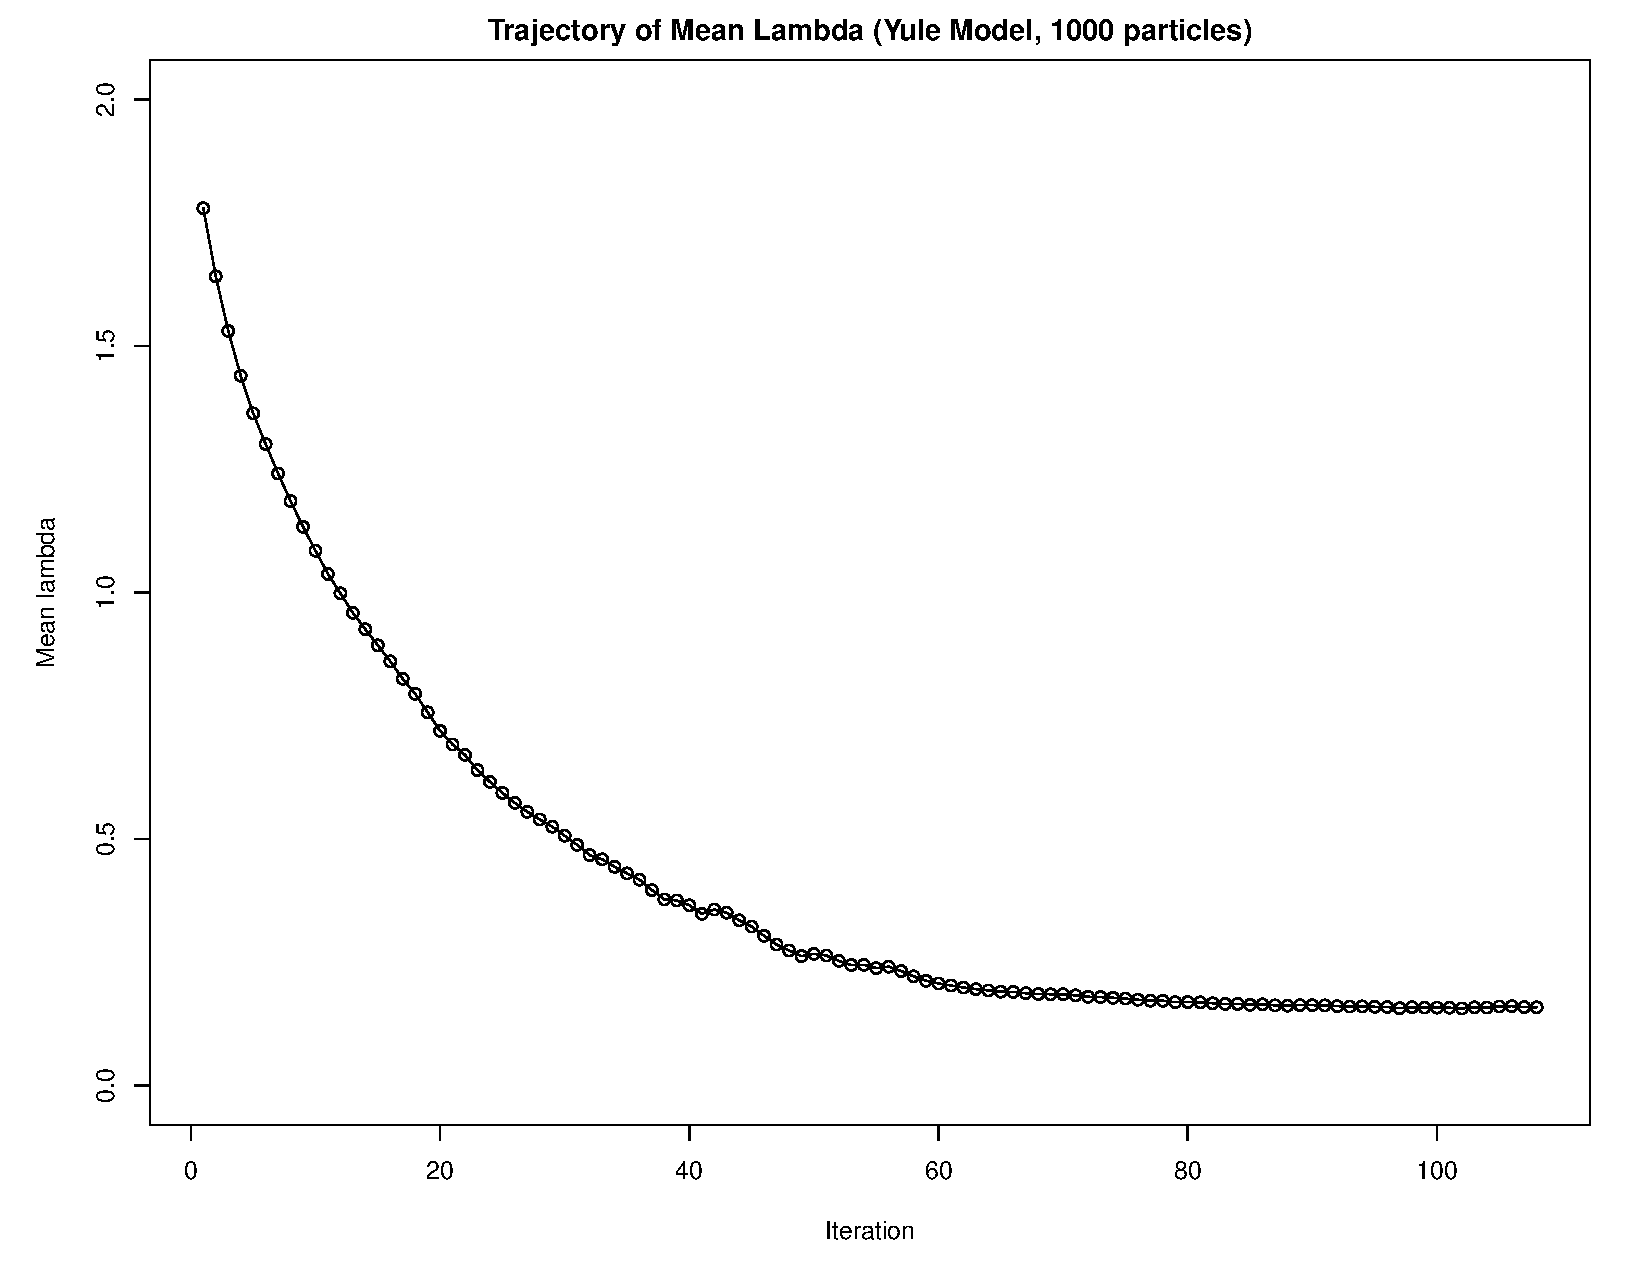
\includegraphics[width=\textwidth]{Yule_Traj_2.pdf}
\caption[Trajectory of lambda (Yule)]{Trajectory of mean lambda for Yule model with 1000 particles.}
\centering
\label{2}
\end{figure}

\begin{figure}[ht]
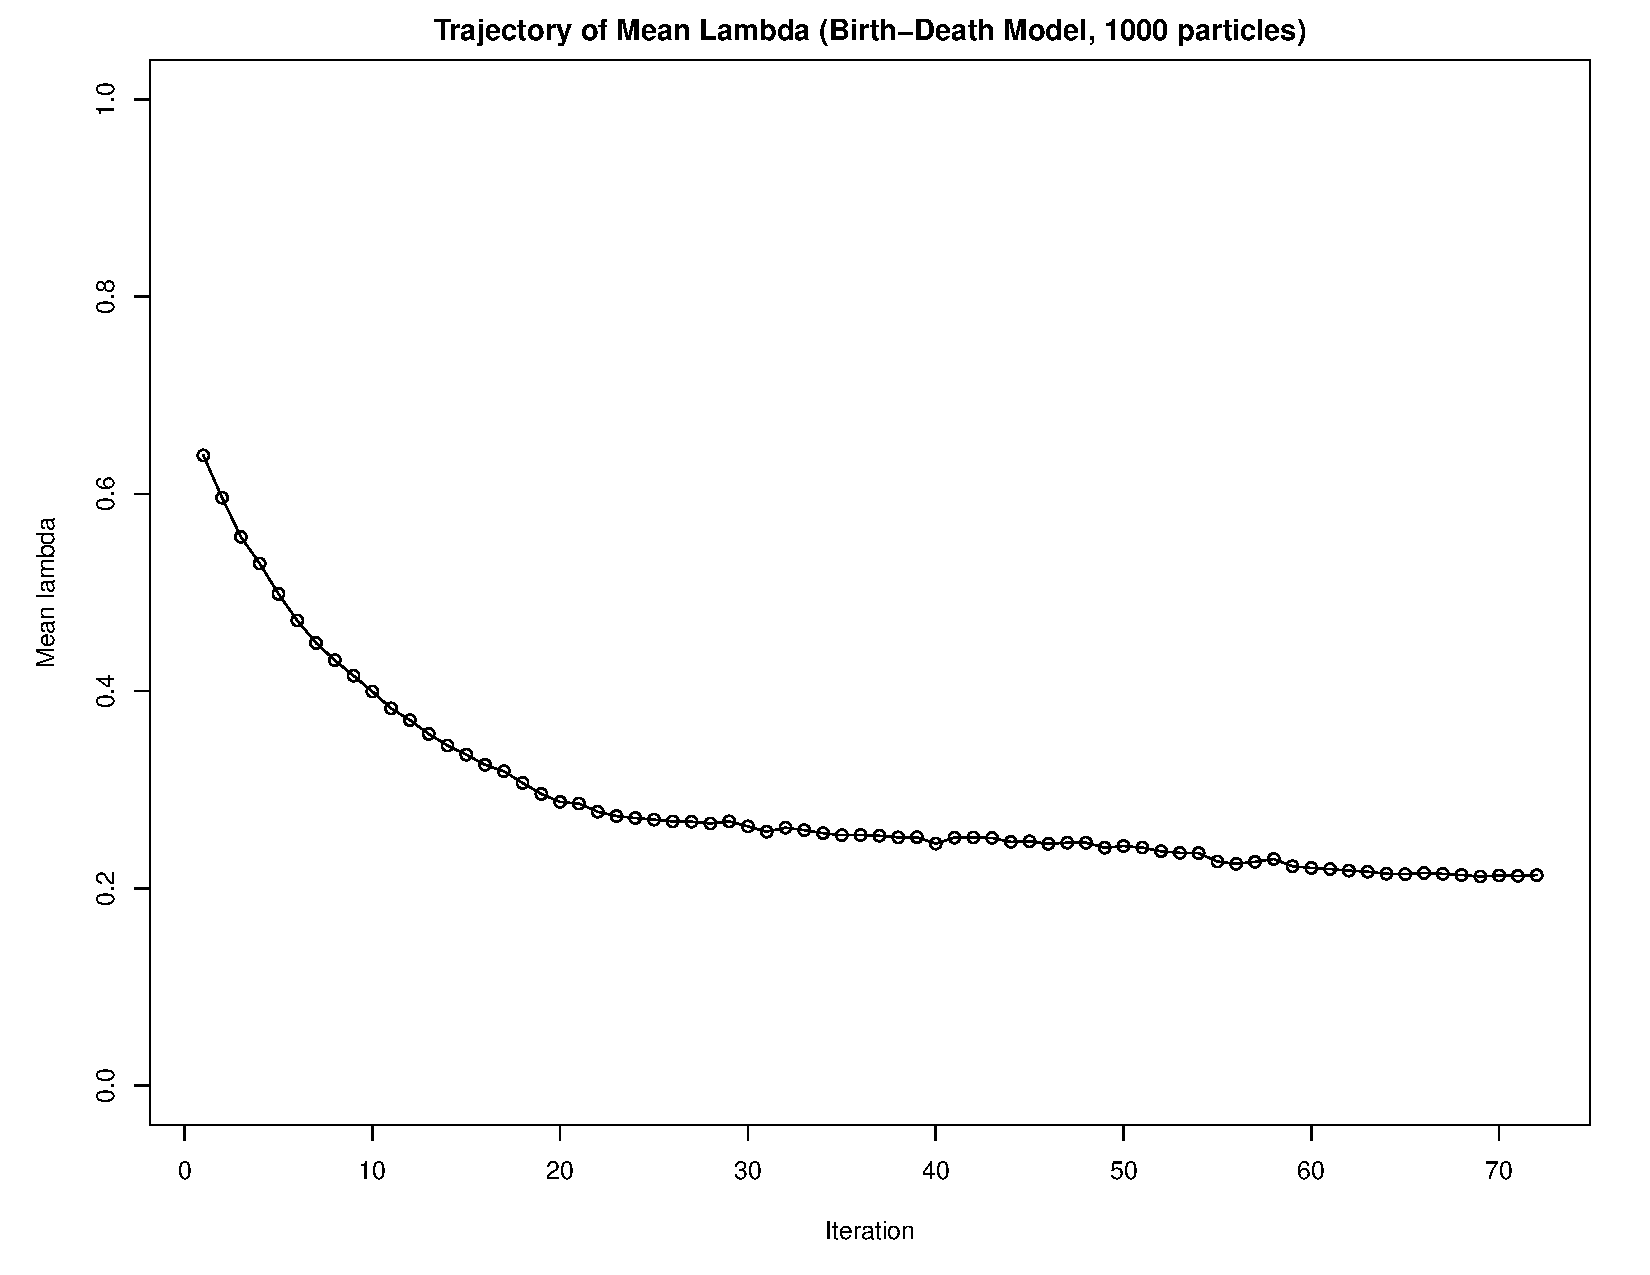
\includegraphics[width=\textwidth]{bd_lambda_traj.pdf}
\caption[Trajectory of lambda (birth-death)]{Trajectory of mean lambda for birth-death model with 1000 particles.}
\centering
\label{3}
\end{figure}

\begin{figure}[ht]
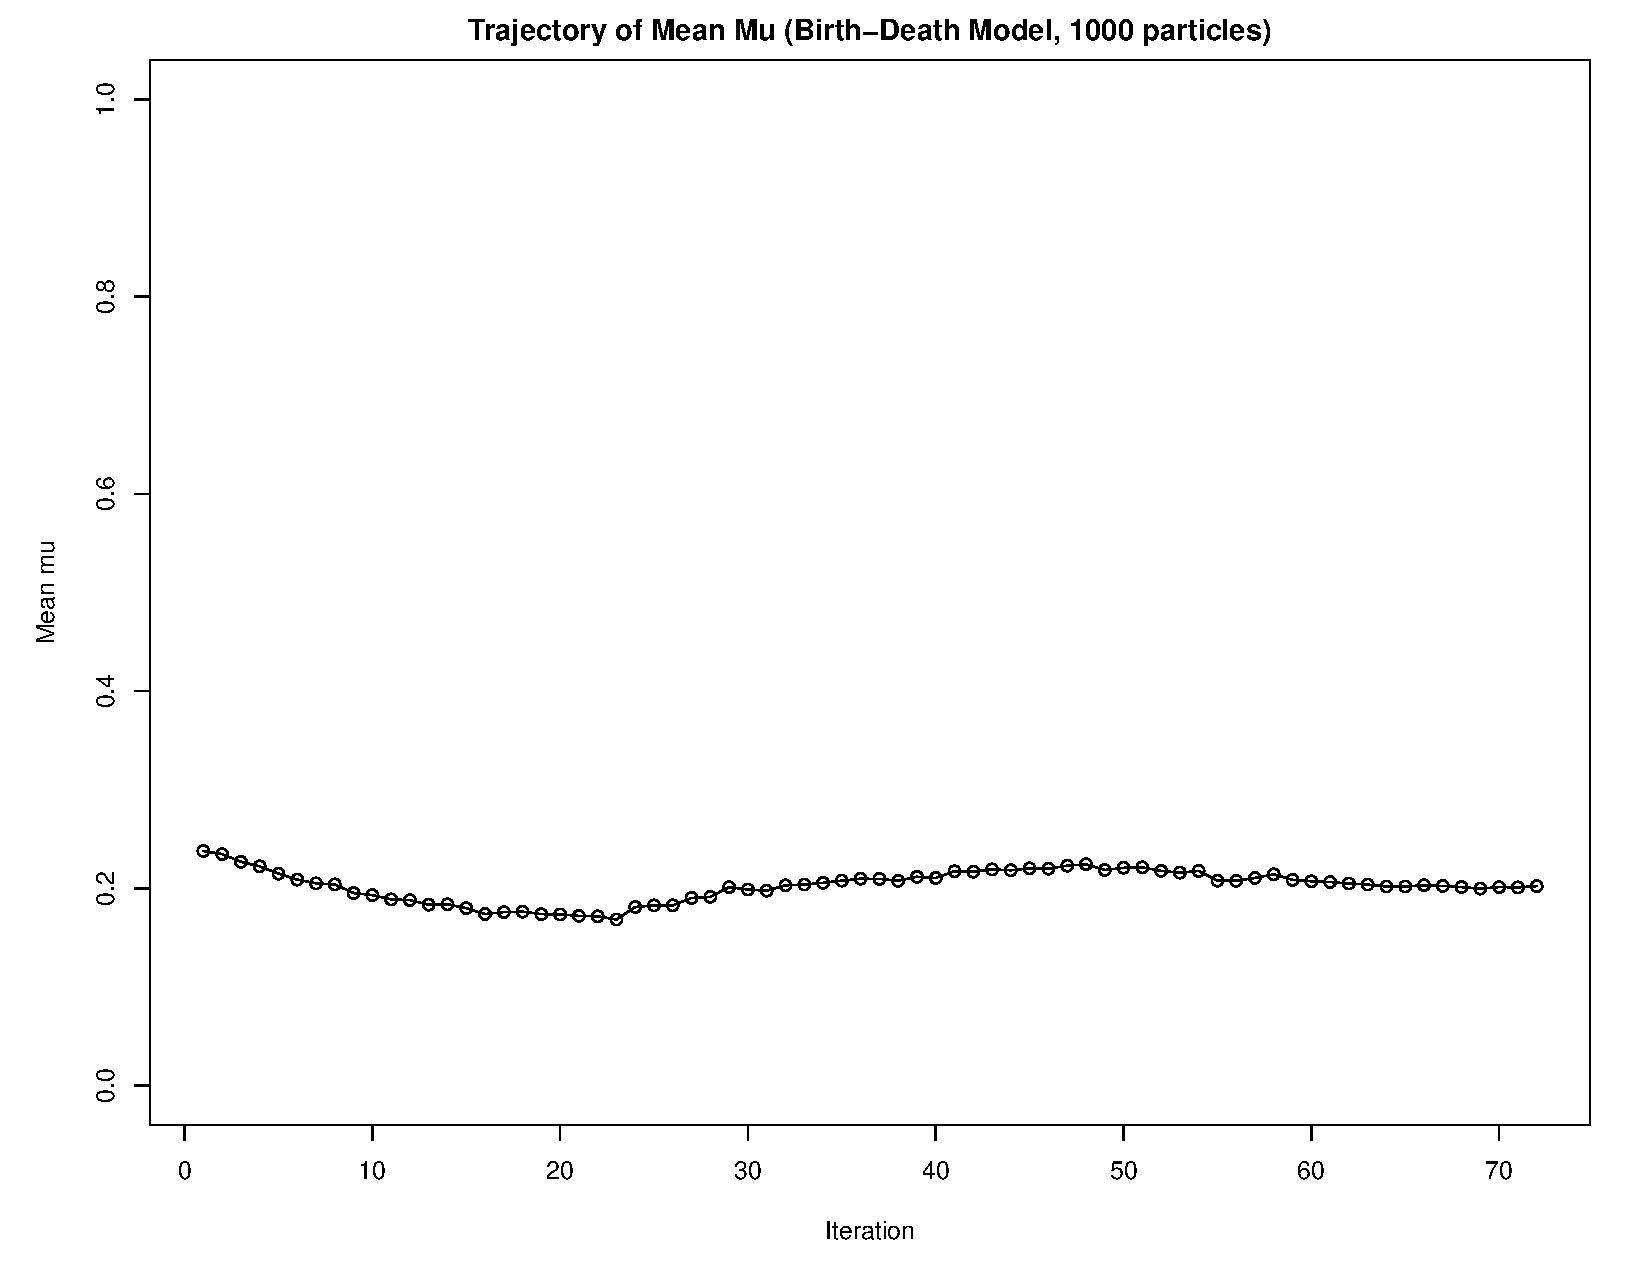
\includegraphics[width=\textwidth]{bd_mu_traj.pdf}
\caption[Trajectory of mu (birth-death)]{Trajectory of mean mu for birth-death model with 1000 particles.}
\centering
\label{4}
\end{figure}

	The plots for lambda show a clear plateau after the initial burn in. Mu, however, does not follow this pattern. This is due to confounding of lambda and mu. As shown by figure~\ref{5}, lambda and mu are moderately confounded with a positive association. In this heat map, the true values of lambda and mu for the observed tree are shown as dashed lines. The confounding of lambda and mu is a limitation of Kaphi when it comes to identifying the effect of mu under the birth-death model.

\begin{figure}[ht]
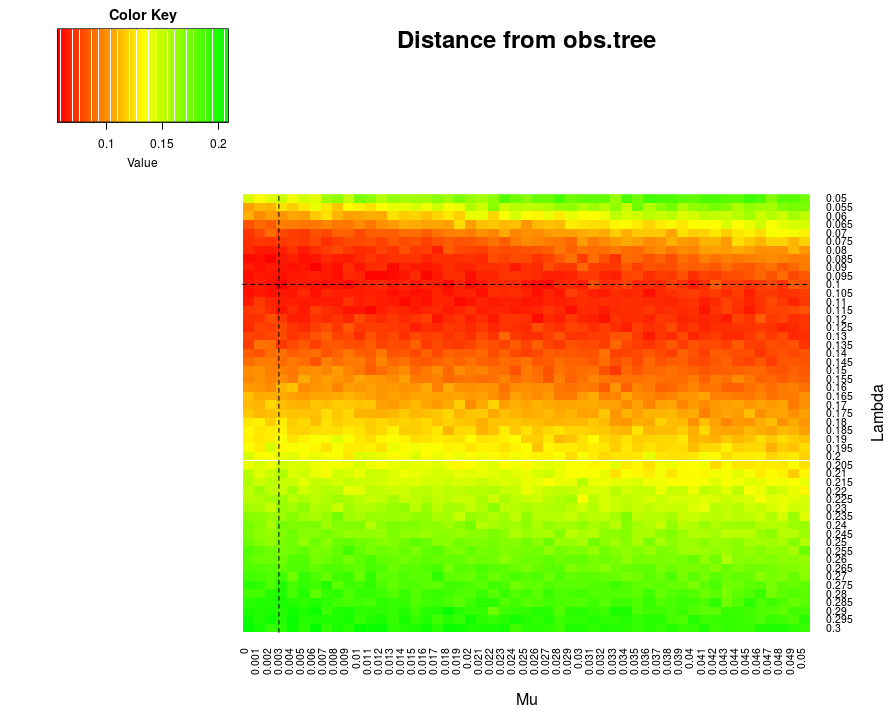
\includegraphics[width=\textwidth]{heatmap.png}
\caption[Heat map]{Heat map showing the distance of pairwise parameter combinations from a tree.}
\centering
\label{5}
\end{figure}

	The next set of plots (figures~\ref{6},~\ref{7},~\ref{8}, and~\ref{9}) are visualizations of the posterior approximations of the parameters at different iterations, compared to the prior distribution. The birth-death plots show the kernel density at every 10 iterations, while the Yule model plots show every 20. This is simply do to the fact that the increased number of iterations of the Yule model would clutter the plot. All 4 figures are similar in that the final density converges sufficiently on the average parameter value. 

\begin{figure}[ht]
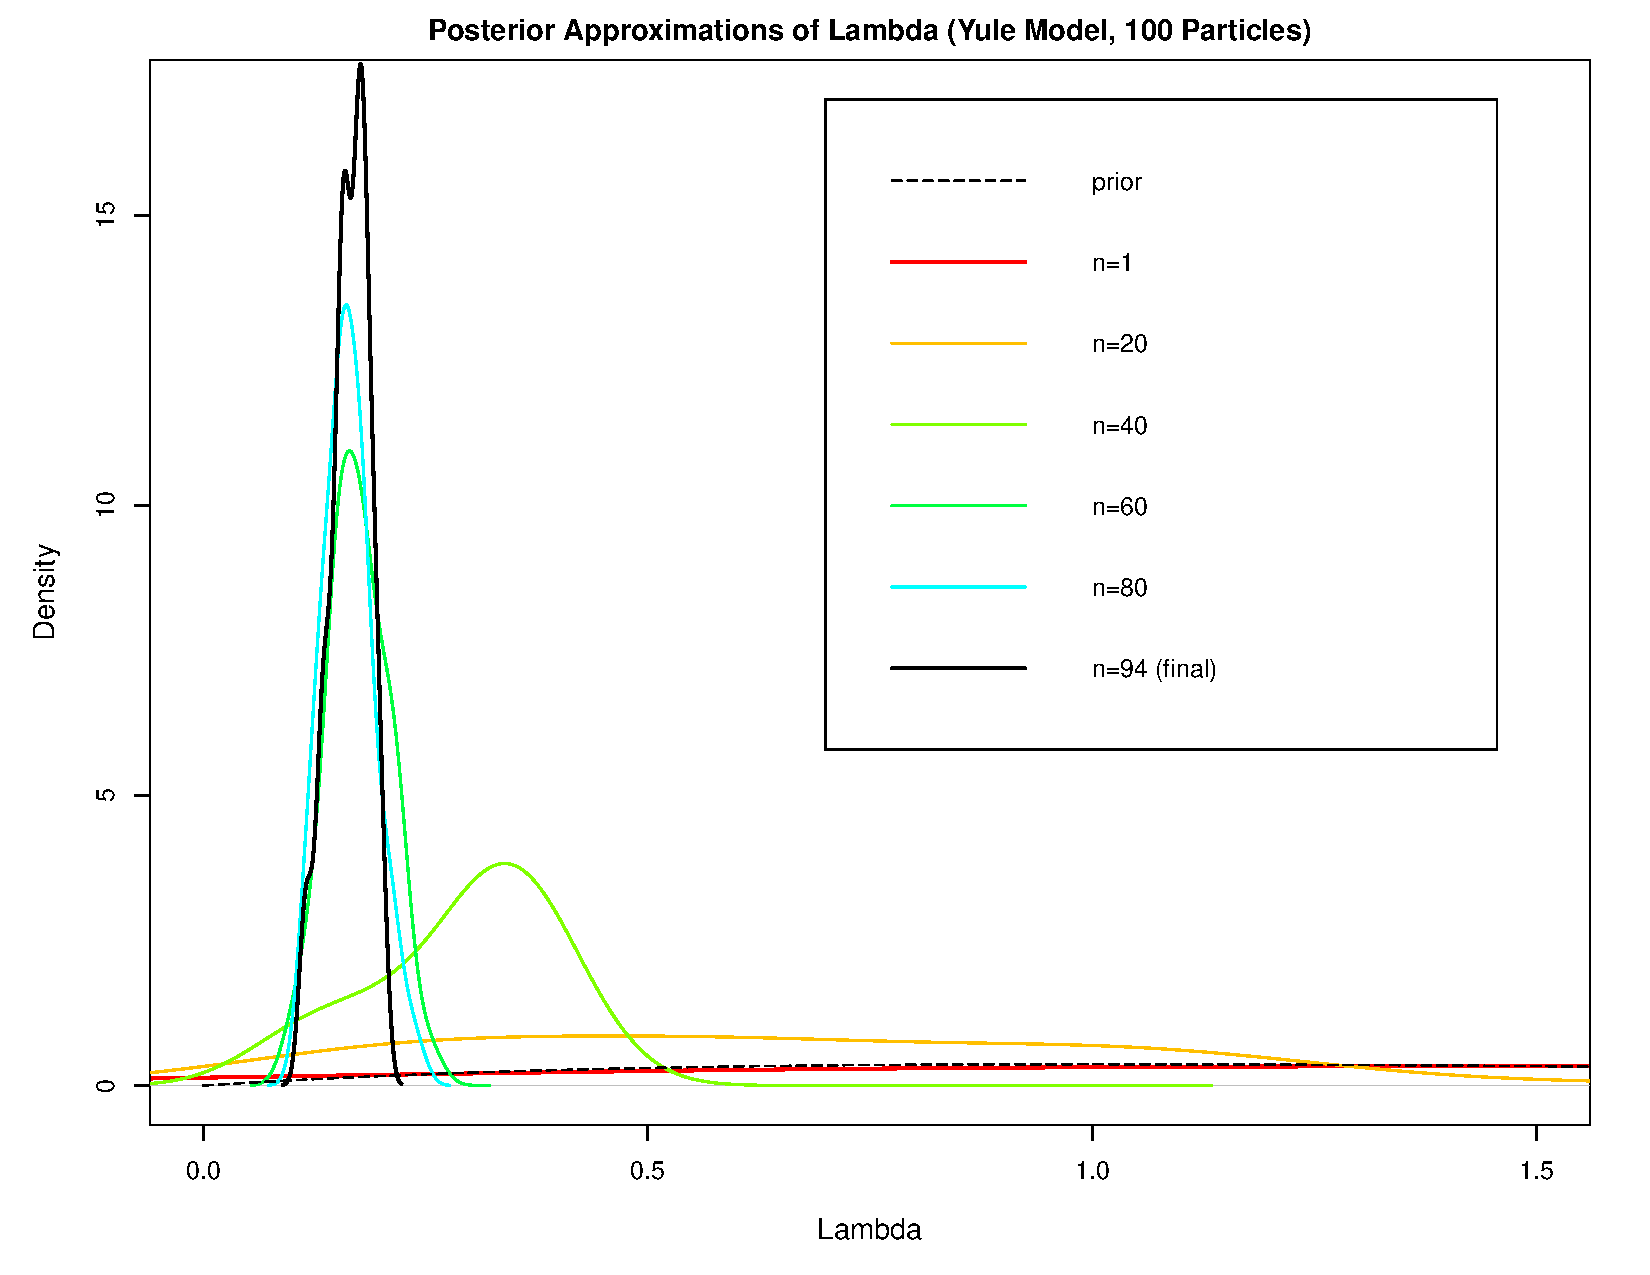
\includegraphics[width=\textwidth]{Yule_Approx_1.pdf}
\caption[Approximation of lambda (Yule, 100 particles)]{Posterior Approximations of Lambda (Yule Model — 100 particles)}
\centering
\label{6}
\end{figure}

\begin{figure}[ht]
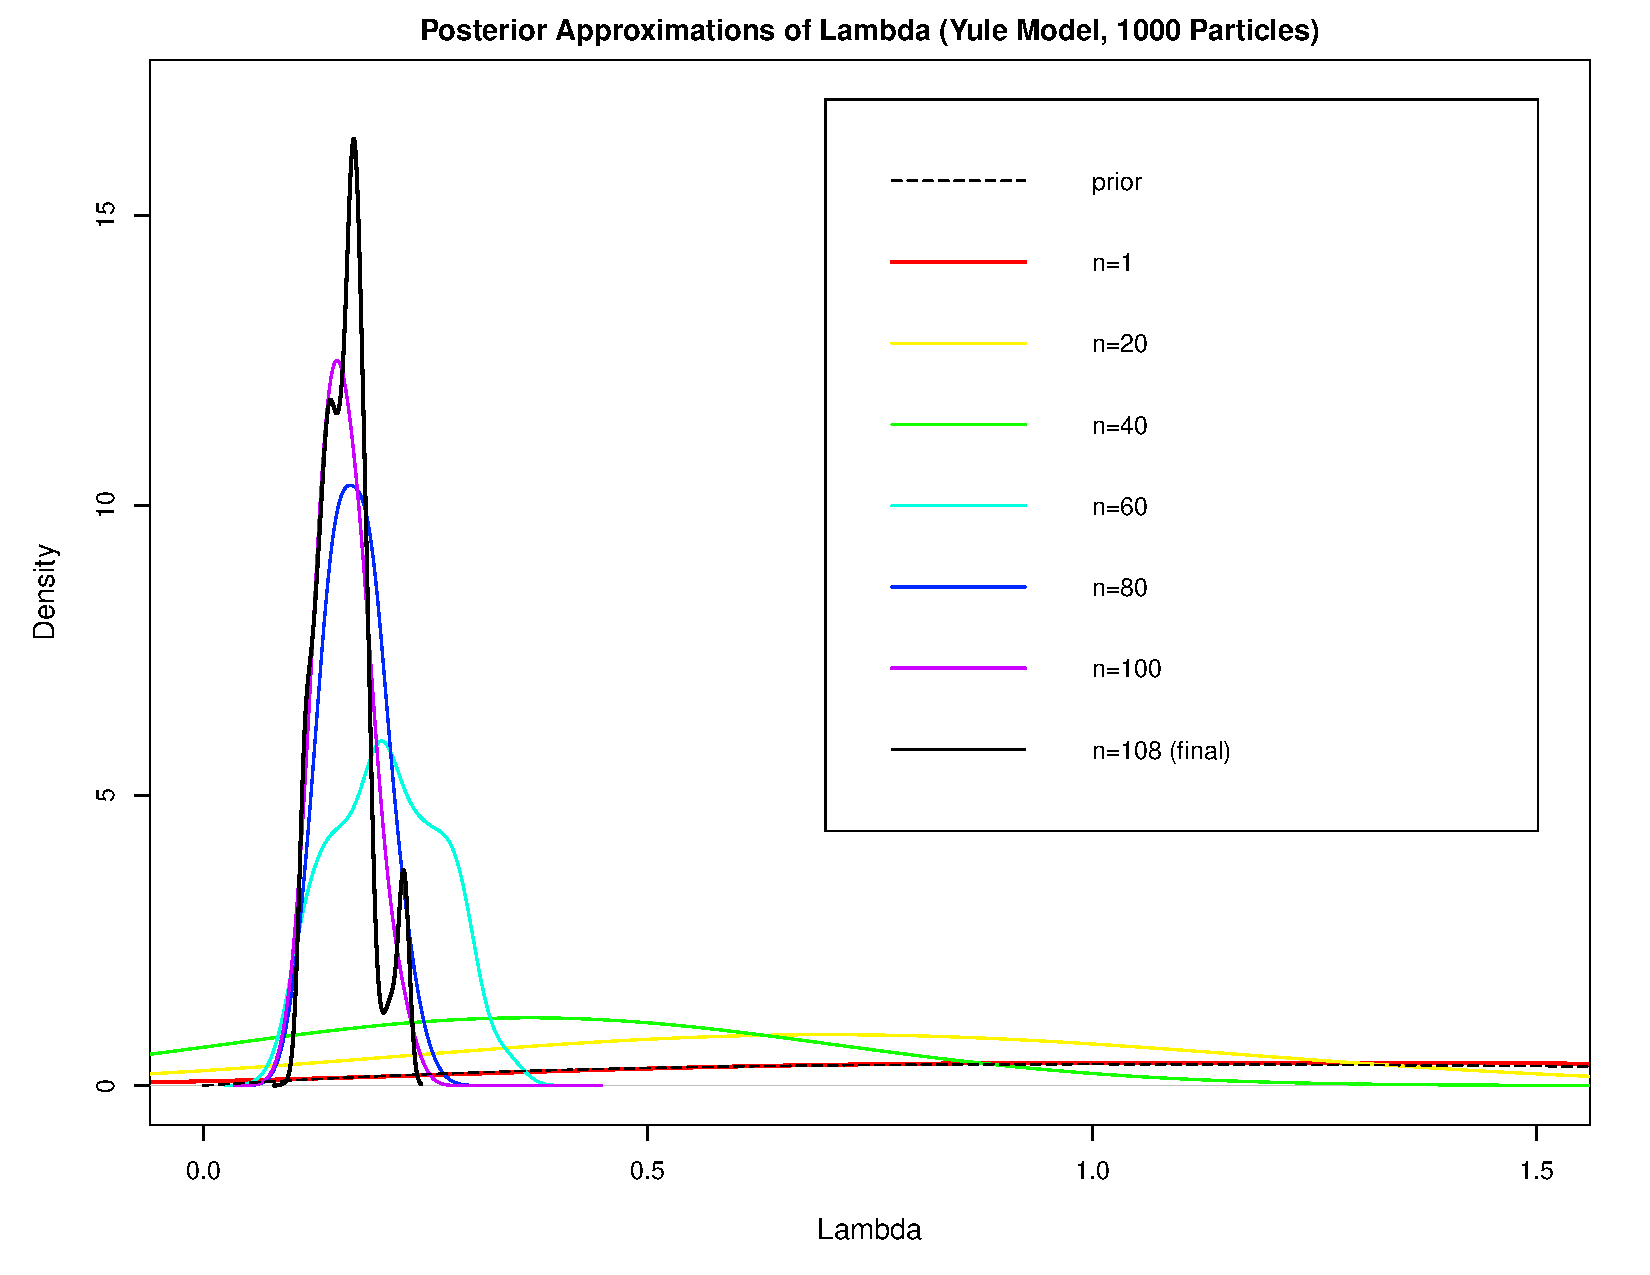
\includegraphics[width=\textwidth]{Yule_Approx_2.pdf}
\caption[Approximation of lambda (Yule, 1000 particles)]{Posterior Approximations of Lambda (Yule Model — 1000 particles)}
\centering
\label{7}
\end{figure}


\begin{figure}[ht]
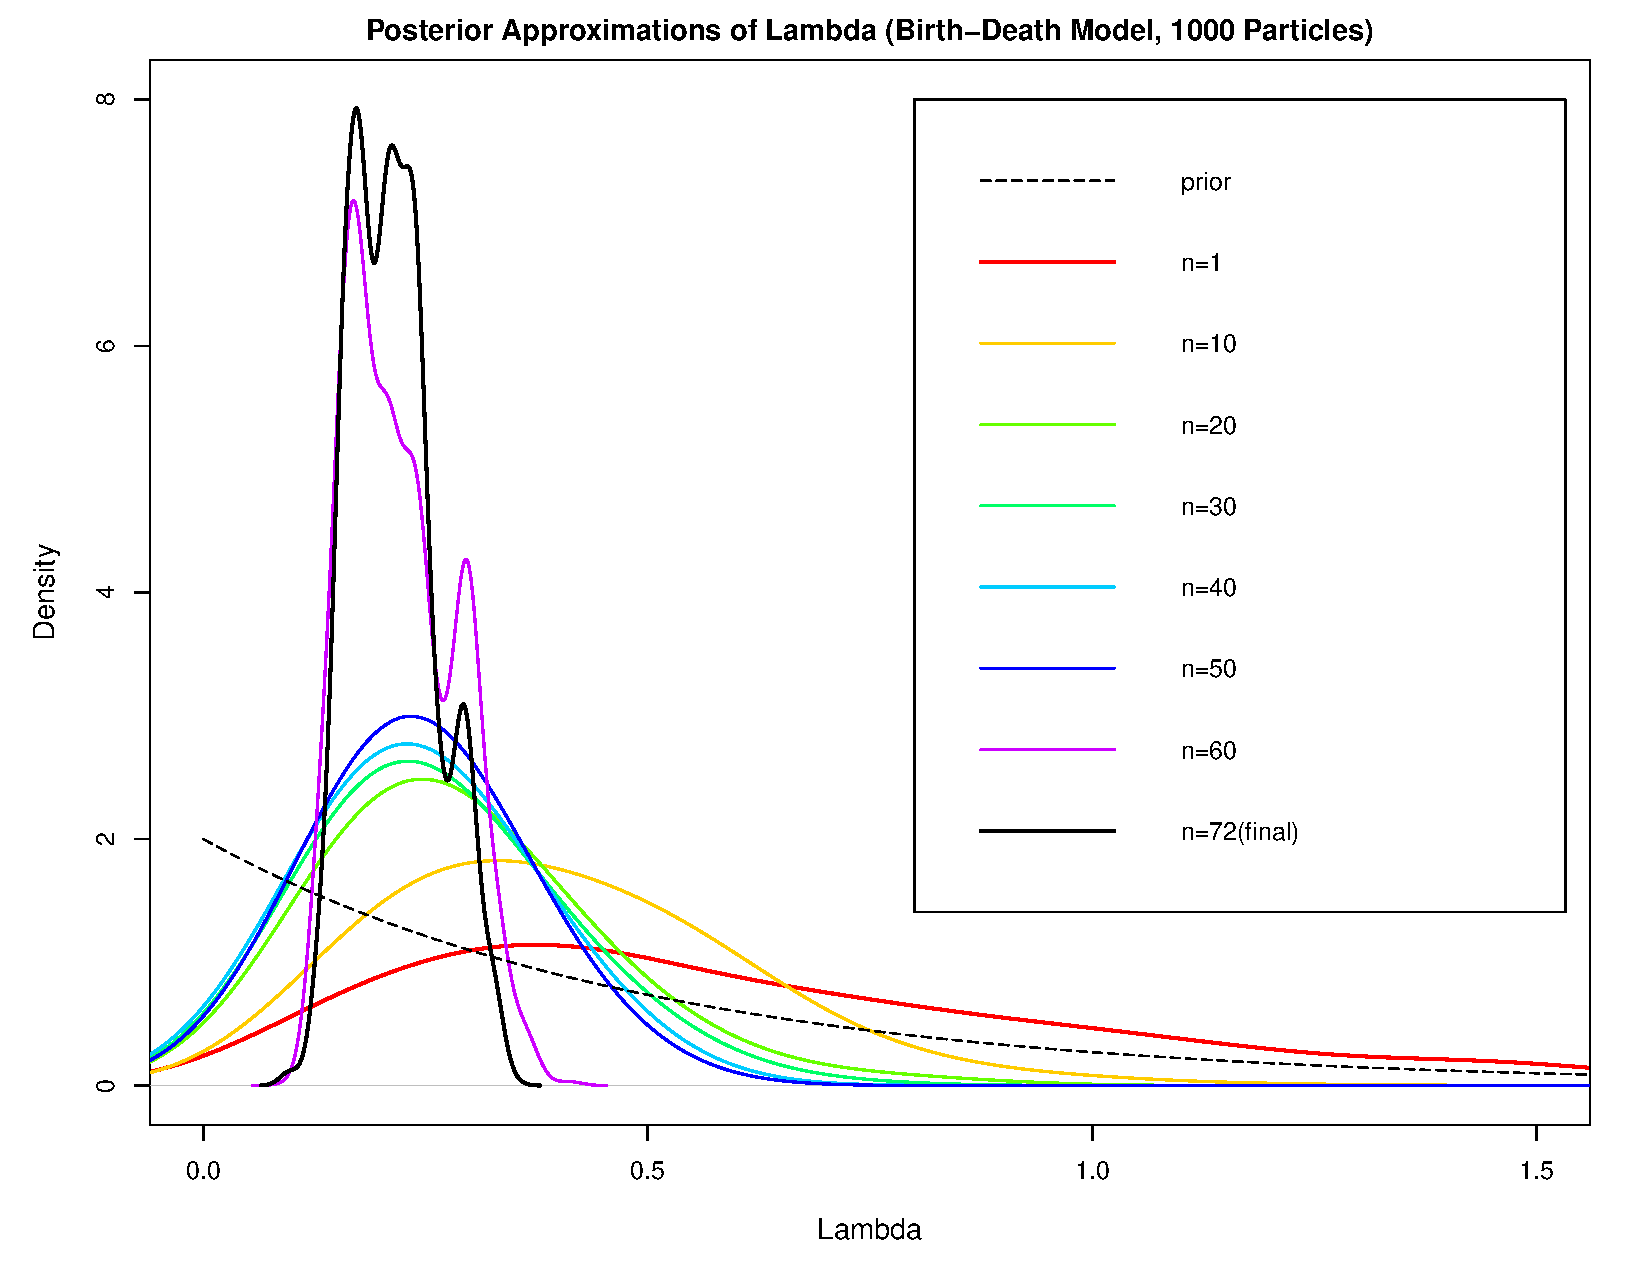
\includegraphics[width=\textwidth]{bd_lambda_approx.pdf}
\caption[Approximation of lambda (birth-death)]{Posterior Approximations of Lambda (Birth-Death Model — 1000 particles)}
\centering
\label{8}
\end{figure}

\begin{figure}[ht]
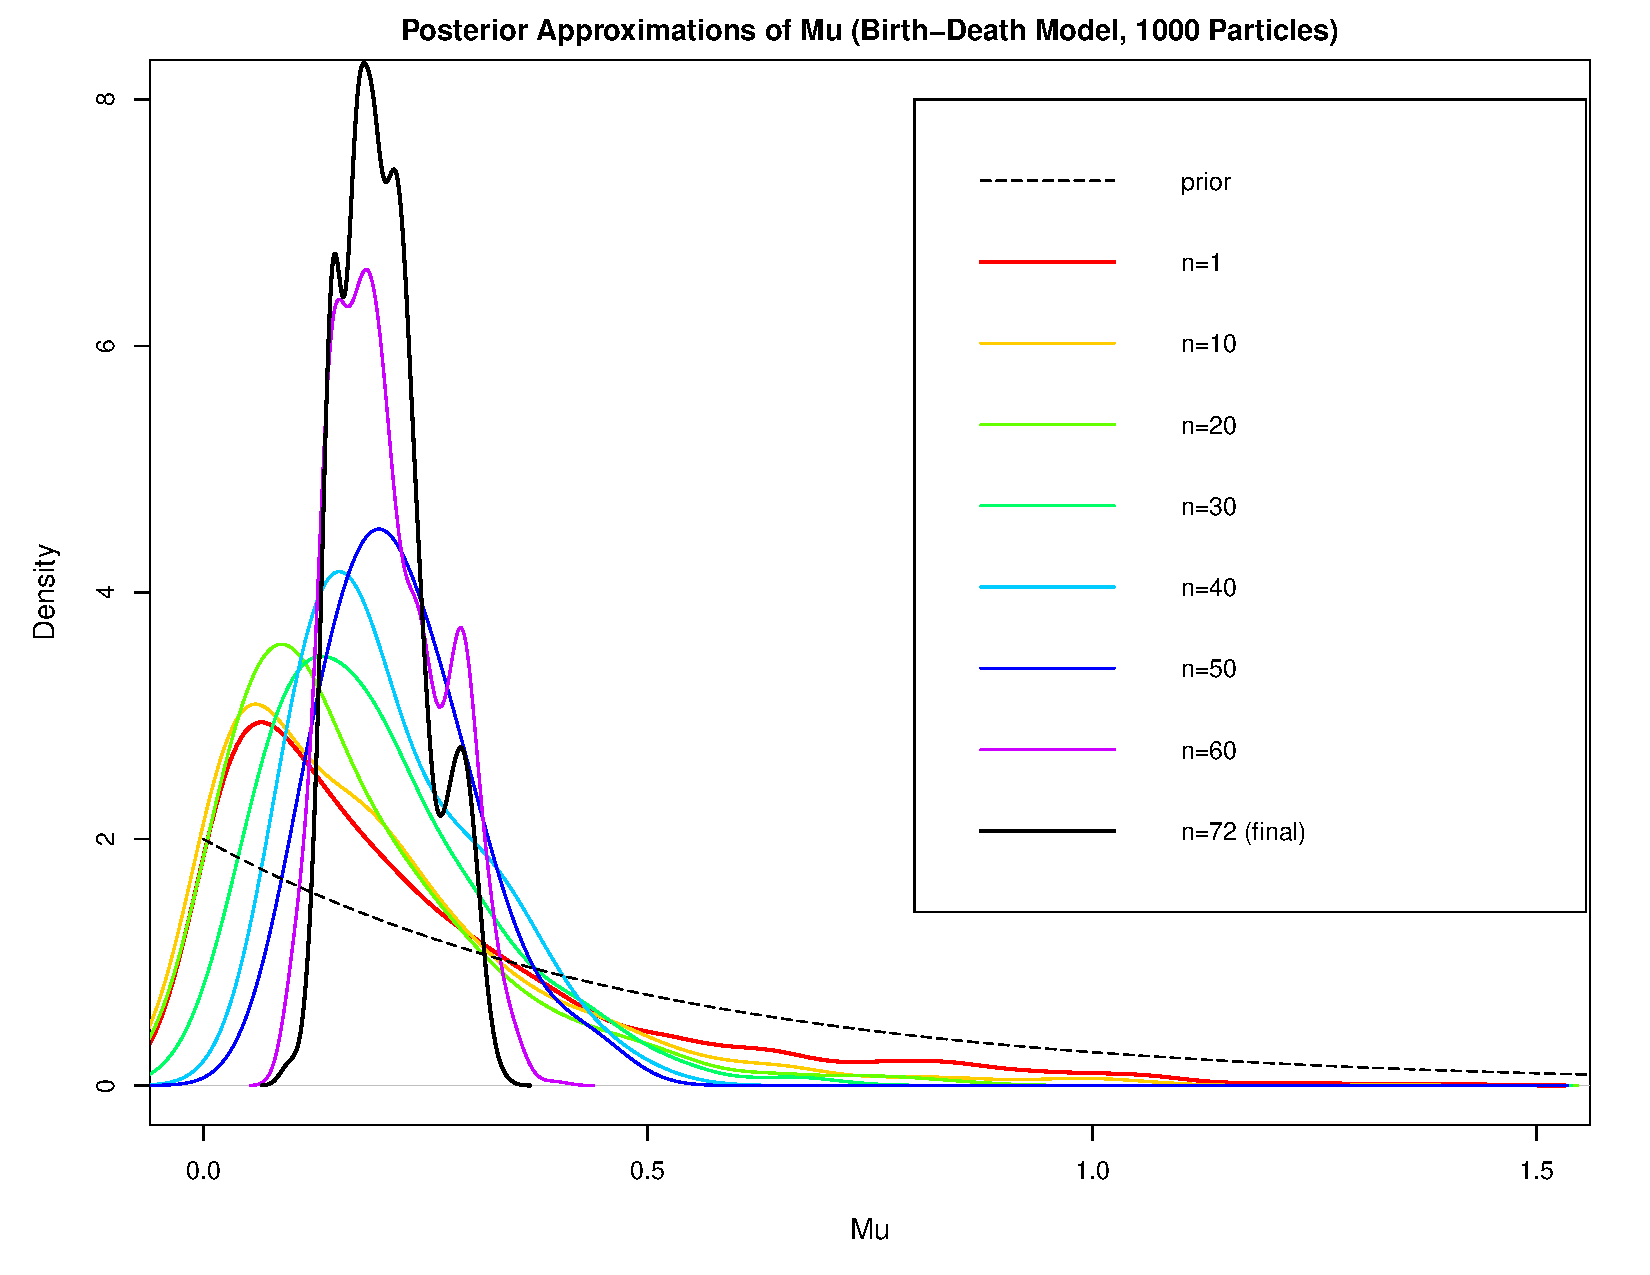
\includegraphics[width=\textwidth]{bd_mu_approx.pdf}
\caption[Approximation of mu (birth-death)]{Posterior Approximations of Mu (Birth-Death Model — 1000 particles)}
\centering
\label{9}
\end{figure}

	These results do not have much meaning on their own, and subsequent experiments are required in order to utilize different methods and data sets to draw meaningful conclusions on the diversification of cyanobacteria (see Recommendations). For example, the software TreePar was used by Marin et al. in their 2016 study of prokaryote phylogenies to perform a rate shift analysis \cite{marin2016timetree}. This involved splitting the evolutionary history of prokaryotes into regions based on their diversification rates \cite{marin2016timetree}. That analysis resulted in 5 rate intervals throughout the 4,180 million years of prokaryote evolution, each with their own values of lambda and mu \cite{marin2016timetree}.

	In that study, the ratio of lambda to mu for the two phylogenies considered were 1.03 and 1.02, respectively. The ratio obtained from this experiment of cyanobacteria was 1.05. This indicates that although their actual values may differ, these three phylogenies show somewhat similar diversification patterns, which is to be expected.

	As mentioned earlier, phylodynamics is a new area of research and is continuing to grow. As methods that estimate diversification parameters become more available, it will be more feasible for researchers to publish diversification parameter estimates with their phylogenies. An increase in the wealth of diversification data will benefit future studies on the effect of ecological factors on species, and the inter-relatedness of parasite and host evolution, to name a couple.

	Despite the lack findings regarding the data studied, the results of this report can speak to Kaphi as a tool for phylodynamic inference. The current standard for fitting models to tree shapes is BEAST (Bayesian Evolutionary Analysis by Sampling Trees). BEAST uses a Metropolis-Hastings Markov Chain Monte Carlo algorithm as the core of it's functionality \cite{drummond2007beast}. This method requires the calculation of exact likelihoods, which is known to be very computationally expensive \cite{sunnaaker2013approximate}. In addition, BEAST uses an MCMC algorithm to sample prior distributions, which as stated earlier is inferior to SMC sampling in the context of ABC \cite{sisson2007sequential}. These factors limit BEAST in the complexity of models and size of trees that it is able to handle. An additional drawback is that BEAST analyses utilize only the branching times of phylogenies, disregarding all information conveyed by the tree topology \cite{drummond2007beast}.

	Currently, there is a call for new software to address the challenges that the field of phylodynamics is facing, including these shortcomings of BEAST \cite{frost2015eight}. As stated previously, Kaphi has solved these issues with the use of an ABC approach and a kernel function for tree comparison. The advantage of using ABC over traditional Bayesian methods is the ability to simulate trees from the model, rather than having to calculate exact likelihoods \cite{sunnaaker2013approximate}. This allows for estimations of a larger set of parameters, giving the ability to use models that are too complex for other methods. 

	ABC methods depend on having a summary statistic that is adept for handling more realistic models \cite{park2016k2}. It has been shown by several different groups that kernel functions are able to provide accurate summary statistics for ABC \cite{mccloskey2016reconstructing}. The kernel method used to measure distance between trees in this study has been proven to outperform many of the commonly used distance metrics, both in and out of an ABC framework \cite{poon2015phylodynamic}.

	As this study has shown, Kaphi was able to overcome the main problems of BEAST all while maintaining exceptional computational performance. The data set at hand, phylum cyanobacteria, is a substantial phylogeny with 684 extant species. In this case, a precise time to completion for each analysis was not determined due to running multiple analyses at once, as well as performing day-to-day tasks on the same machine. However, these analyses all completed in under 12 hours at most. Since this analysis, Kaphi has implemented parallelization of SMC routines, which has further increased the speed of the program. Initial tests show a 3X reduction in computation time for a simulated Yule model with 1000 particles \cite{poon2017kaphi}. 


% Conclusions %
\section{ Conclusions}
	The results obtained from the analyses performed have proven to be purely exploratory. Much more work must be completed before a comprehensive picture of cyanobacteria speciation patterns can be determined. One conclusion that is able to be drawn from the data is that cyanobacteria diversification, as determined in the report, is largely similar to prokaryotes as a whole. This is due to similar ratios of lambda to mu for the average final values. This is just the beginning of this comparison, as different approaches can further validate this association. However, it is expected that cyanobacteria diversification will approximately resemble that of prokaryotes since it is a member of this greater group.
    
    For the bulk of my discussion, I turned to evaluating Kaphi as a tool for phylodynamic inference. First an foremost, Kaphi boasts functionality that surmounts the issues of it's main competitor, BEAST. The ABC-SMC method is more practical than previously proposed phylodynamics approaches as it is capable of handling more complex models. Any increase in the realism of models is a huge step forward for making inferences. This is especially true for the many sophisticated epidemiological models, such as those used to simulate transmission networks within an infected population.
    
    The kernel method described in this paper is another advantage of Kaphi. This method was created specifically for use in phylodynamic inference in an ABC framework. The method does not lean one way toward topology or branch length measures, but rather a combination of the two. For these reasons, the Kernel-embedded ABC-SMC approach of Kaphi is functionally superior to other methods of uncovering biological patterns from phylogenetic trees.
    
    One last conclusion to be drawn from this analysis of Kaphi is that the efficiency of the program shows great promise for ease of analysis. Although a proper run-time analysis was not performed, Kaphi performed remarkably well in the handling of this large phylogeny. This finding, paired with newly implemented parallel processing abilities, demonstrates the efficiency of Kaphi analyses.
    

% Recommendations %
\section{ Recommendations}
	As was already mentioned in the discussion and conclusions, there is simply not enough data to draw conclusions about the cyanobacteria phylogeny. At present time, few diversification rates are known from only a handful of analyses. In order to uncover patterns in cyanobacteria diversification, many more experiments must be run. Continued work on this study should consider two main aspects:
    
\textbf{1. Compare to Different Methods}\\
	The parameter values obtained from these preliminary analyses should be compared to those obtained from other methods. This will help cross-validate results or highlight inconsistencies.

\textbf{2. Explore Variation in Kaphi}\\
	There is still much to explore with using Kaphi to infer phylodynamic relationships. Kaphi development is on track to validate more complex models of diversification such as Binary State Speciation and Extinction (BiSSE) and Quantitative State Speciation and Extinction (QuaSSE) models. The newly implemented parallel processing abilities will also aid future experiments by considerably increasing computational efficiency. Regardless, there are still limitless combinations of prior and proposal distributions, SMC settings, and distance metrics, all of which can be optimized by continuing to explore their effects on the resultant parameter values.

    
\newpage

% References %
\bibliographystyle{apacite}
\bibliography{wkrpt3.bib}
\newpage


% Appendix A %
\tocsection{Appendix A -- YAML Configuration Files}
YAML configuration files used for Kaphi analyses.
\begin{minted}[
    autogobble,
    frame=lines,
    linenos=true,
  ]{yaml}
  # Yule model configuration
    priors:
      lambda:
        dist: 'gamma'
        hyperparameters:
        - shape: 2.0 # kappa
        - rate: 1.0  # theta
    constraints:
      - ''
    proposals:
      lambda:
        dist: 'norm'
        parameters:
        - mean: 0.0
        - sd: 0.1
    smc:
      nparticle: 1000
      nsample: 5
      ess.tolerance: 50.0
      final.accept.rate: 0.05
      final.epsilon: 0.05
      quality: 0.95
      step.tolerance: 1.e-4
    distances:
      'kernel.dist':
        weight: 1.0
        decay.factor: 0.2
        rbf.variance: 100.0
        sst.control: 1.0
        norm.mode: 'NONE'
\end{minted}

\begin{minted}[
    autogobble,
    frame=lines,
    linenos=true
  ]{yaml}
  # Birth-Death model configuration
    priors:
      lambda:
        dist: 'gamma'
        hyperparameters:
          - rate: 2.0
          - shape: 1.0
      mu:
        dist: 'gamma'
        hyperparameters:
          - rate: 2.0
          - shape: 1.0
    constraints:
      - 'mu < lambda'
    proposals:
      lambda:
        dist: 'norm'
        parameters:
          - mean: 0
          - sd: 0.1
      mu:
        dist: 'norm'
        parameters:
          - mean: 0
          - sd: 0.1
    smc:
      nparticle: 1000
      nsample: 5
      ess.tolerance: 50.0
      final.accept.rate: 0.05
      final.epsilon: 0.05
      quality: 0.95  
      step.tolerance: 1.e-4
    distances:
      'kernel.dist':
        weight: 1.0
        decay.factor: 0.2
        rbf.variance: 100.0
        sst.control: 1.0
        norm.mode: 'NONE'
\end{minted}

% Appendix B %
\tocsection{Appendix B -- Phylogeny of Cyanobacteria}
The cyanobacteria phylogeny is a subtree of a comprehensive tree of prokaryotes \cite{marin2016timetree}. These visualizations are to give a sense of the size of the tree. The complete list of species and GenBank accession numbers can be found in the report Github repository (\url{github.com/MathiasRenaud/wkrpt-3}).

\begin{figure}[ht]
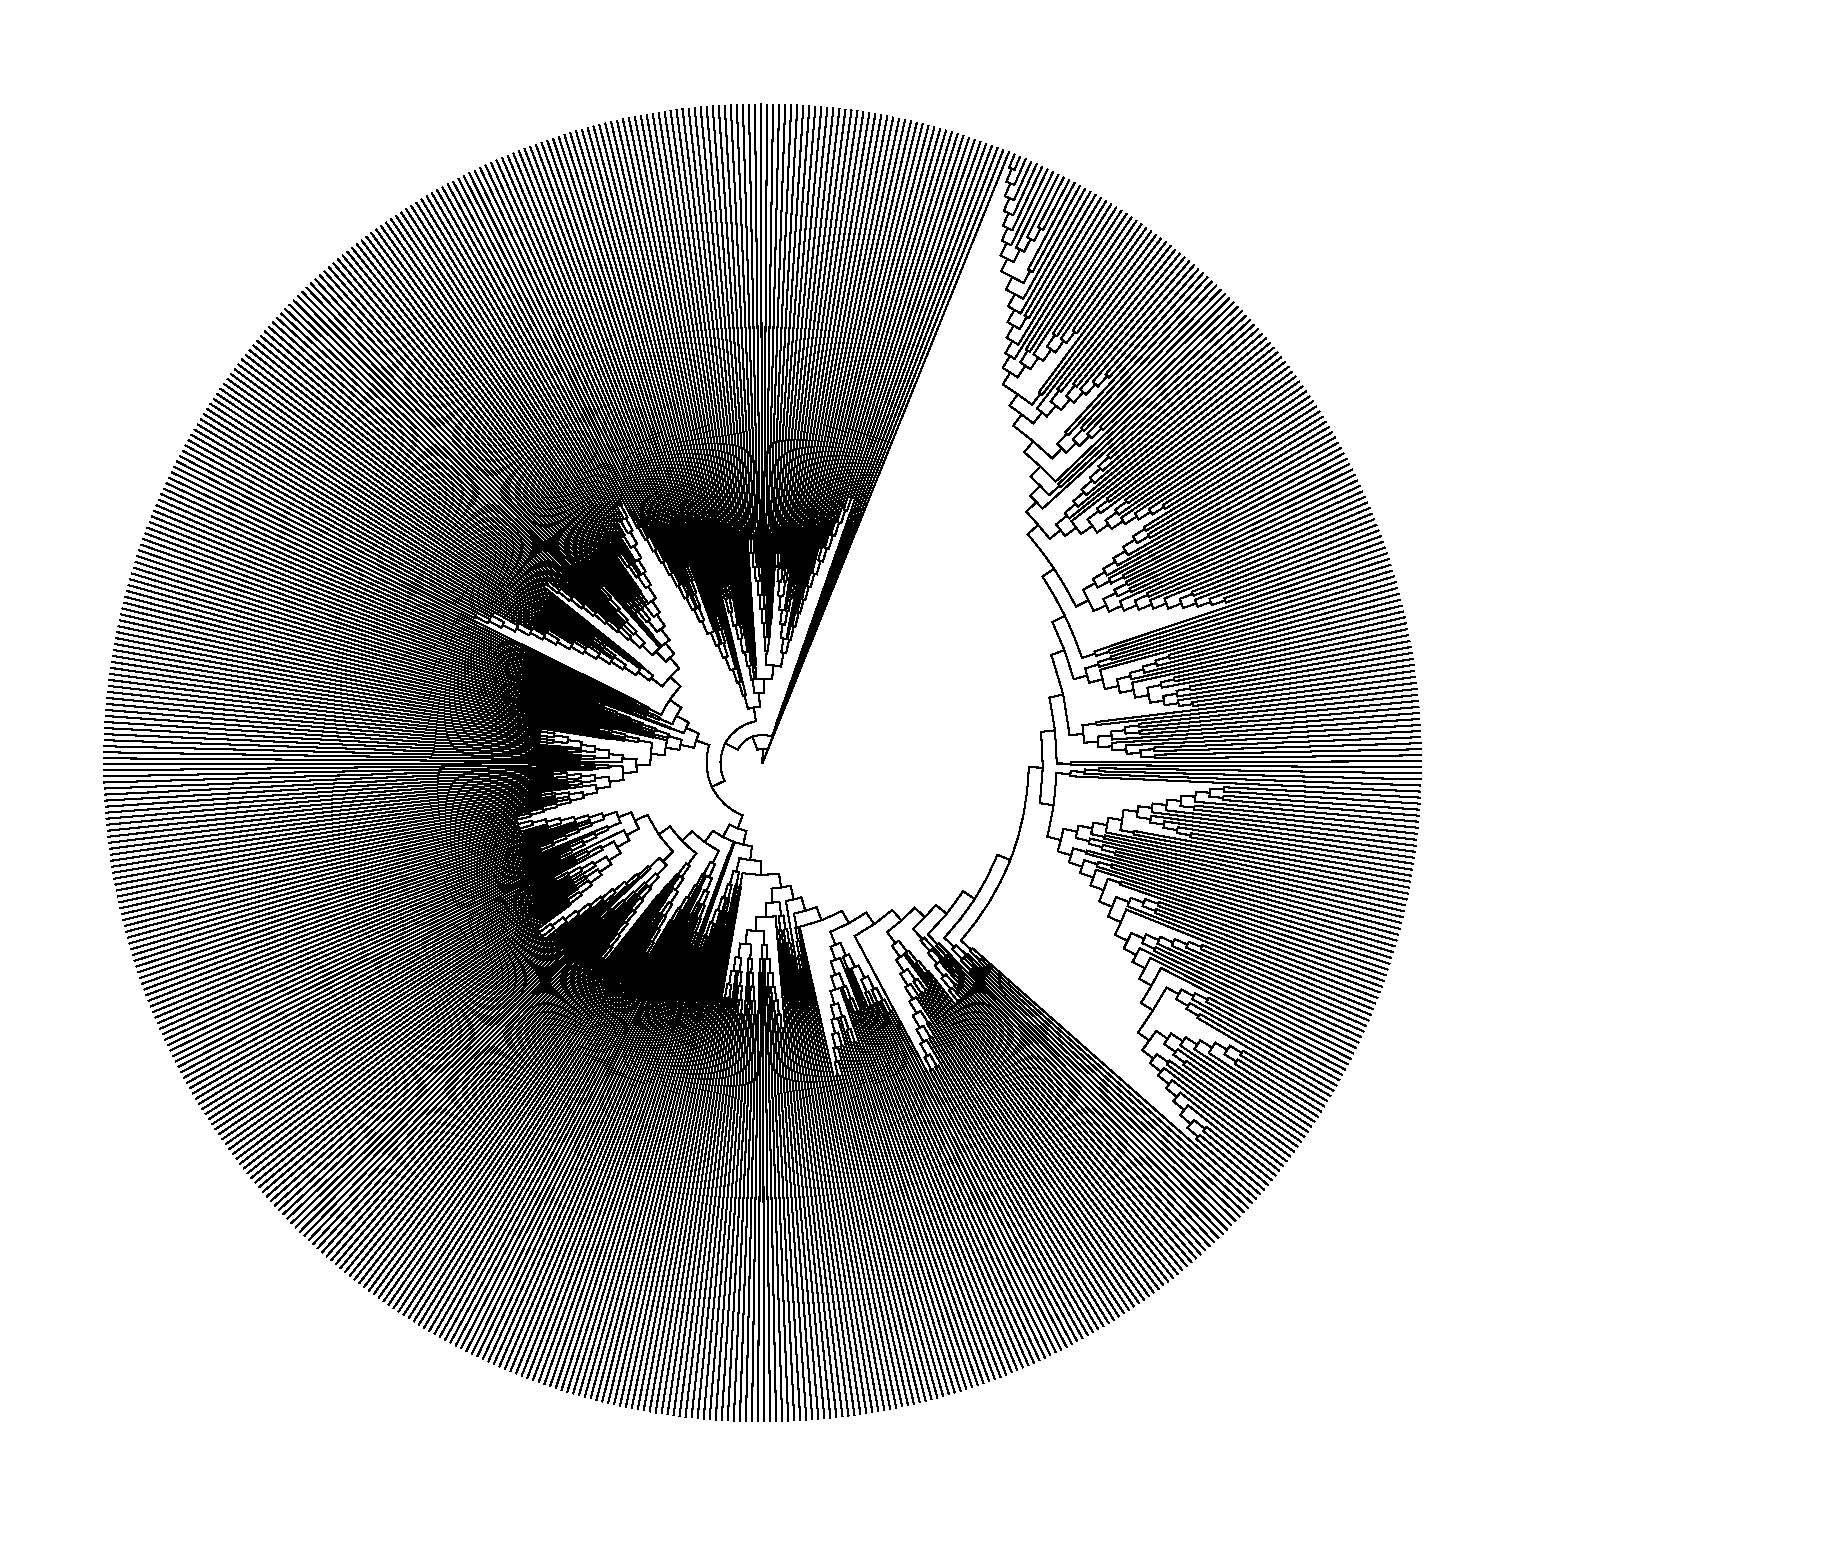
\includegraphics[width=\textwidth]{cyano.pdf}
\caption[Circular Cyanobacteria Tree]{Circular cyanobacteria tree.}
\centering
\label{10}
\end{figure}

\begin{figure}[ht]
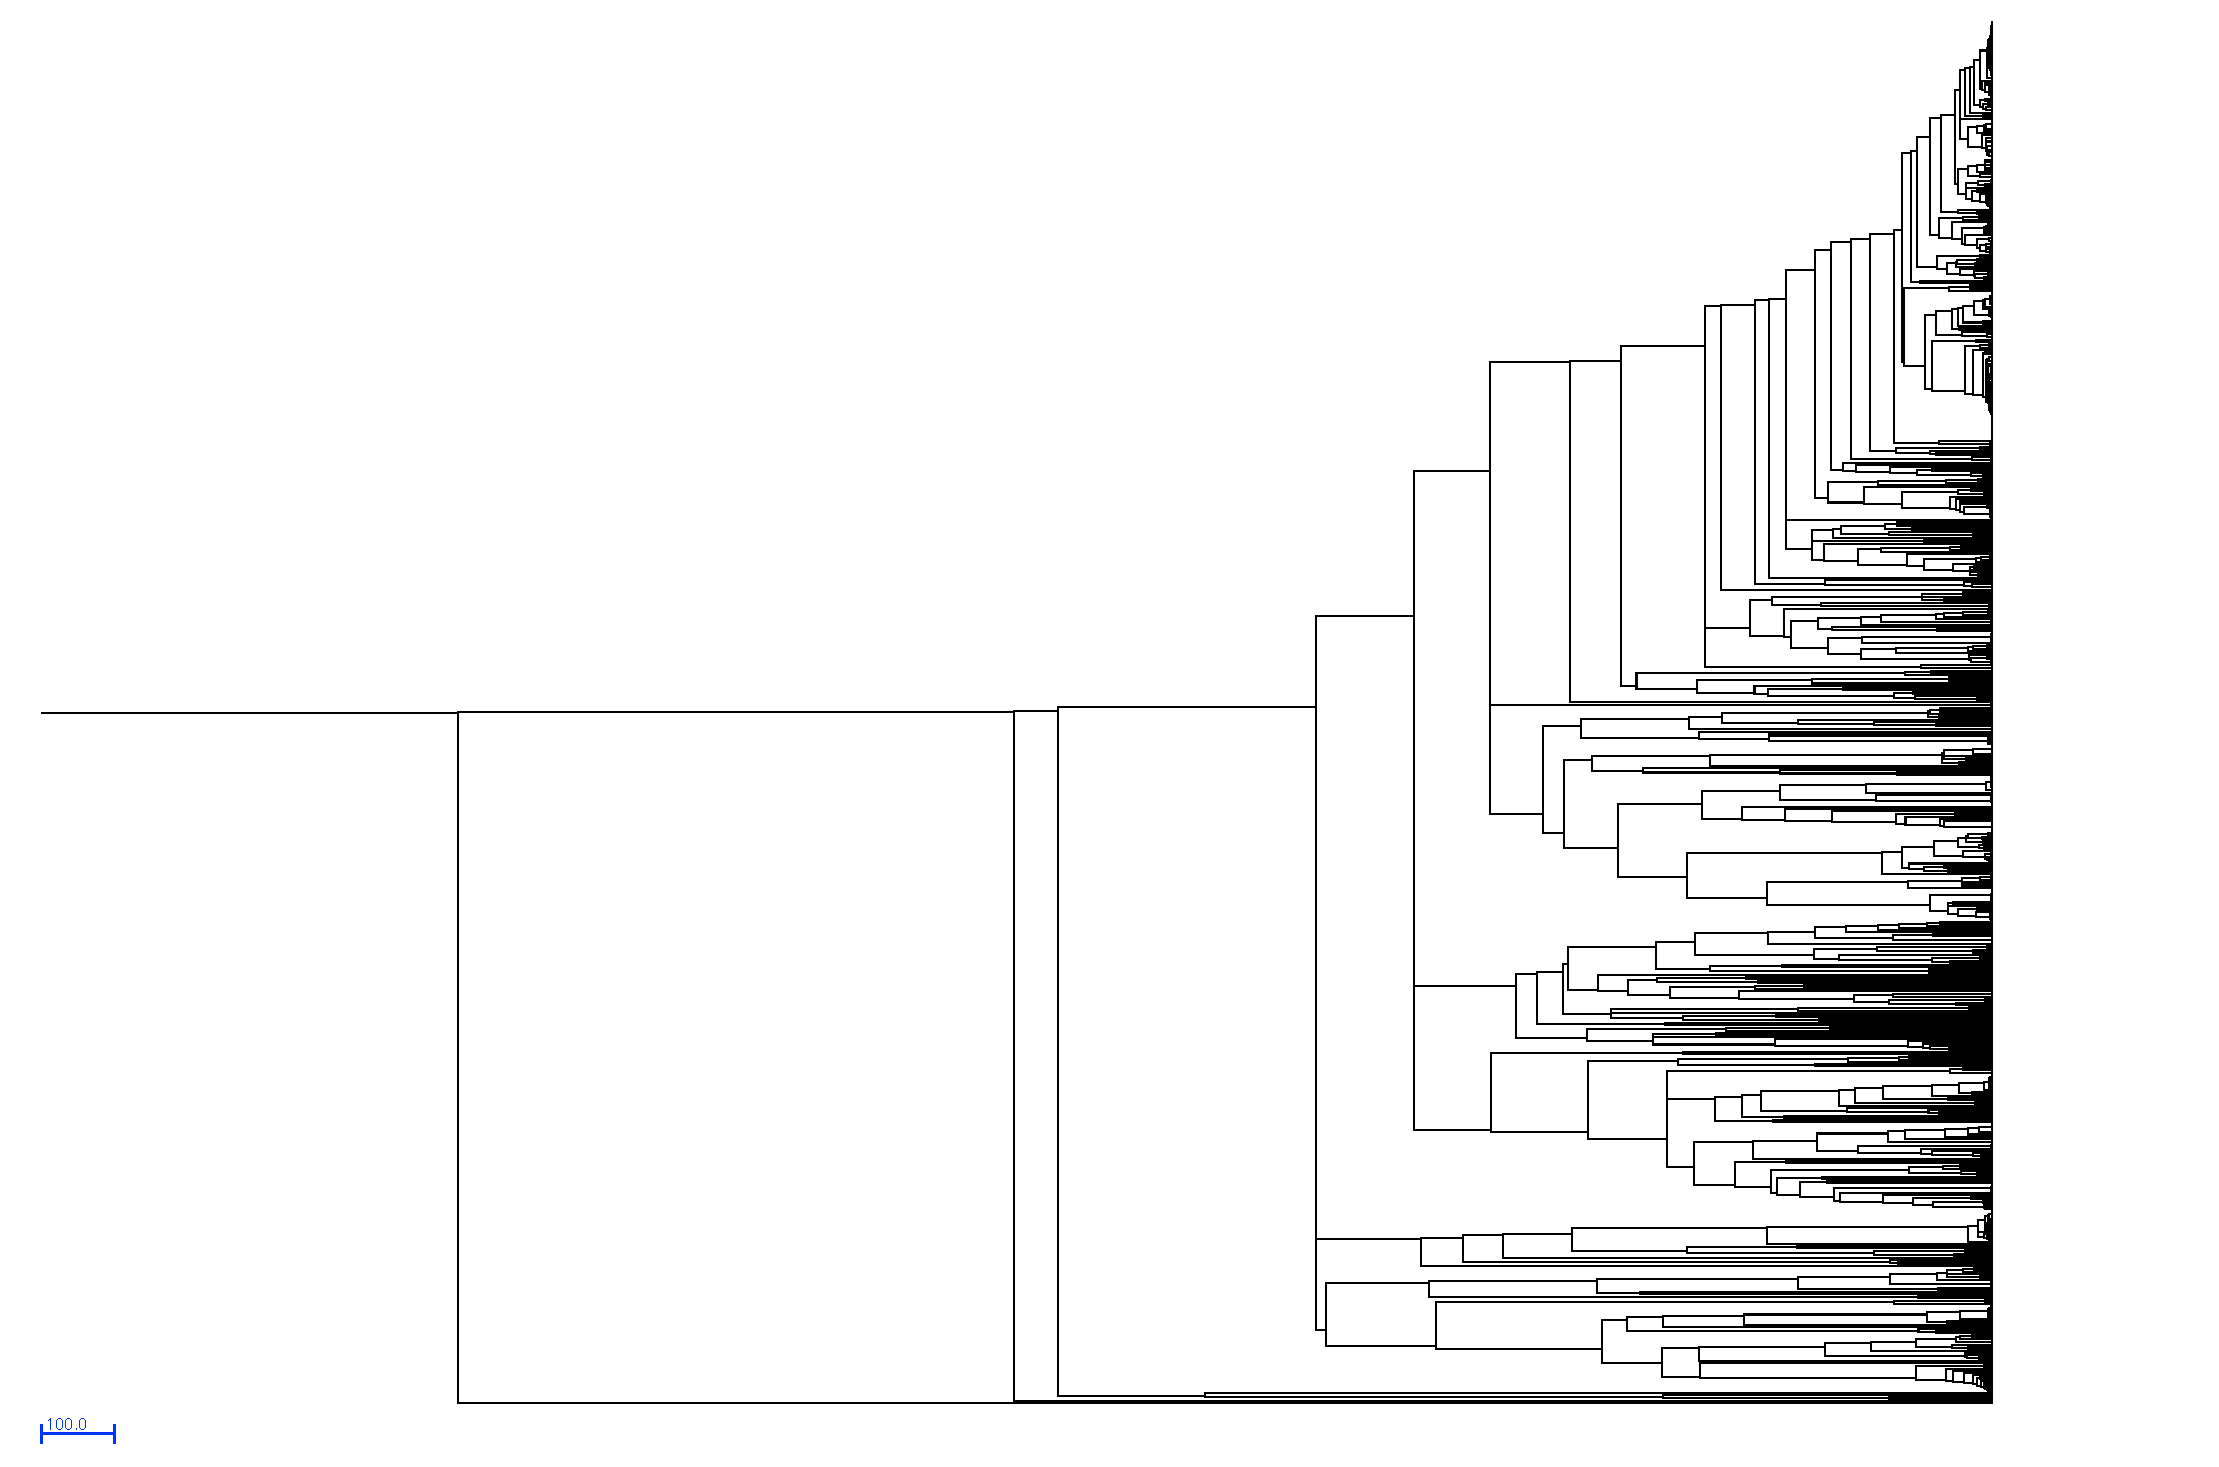
\includegraphics[width=\textwidth]{cyano_rect.pdf}
\caption[Rectangular Cyanobacteria Tree]{Rectangular cyanobacteria tree.}
\centering
\label{11}
\end{figure}

\newpage
\end{document}